
Producer node selection on the Catalyst network is critical to the consensus algorithm as it ensures that a random sub-set of nodes is randomly and fairly selected to produce the next ledger state update. Unlike a majority of tradition blockchain consensus algorithms, Catalyst requires a verifiable list of nodes that have the authority to participate in any given ledger cycle. This verfiable list of the author nodes is utilised througout the consensus algorithm and is used to determine which nodes provide valuable work for the network.  \\

While it would be trivial to select nodes based on some pre-determined value e.g. their peer ID, this mechanism is not wholly random and nodes could manipulate these ID's in order to guarantee themselves a better chance of becoming a producer for a given cycle. As the Catalyst consensus algorithm is reliant on being fair and ensuring that the probability of any one worker node has the same probability as all other to be selected from cycle to cycle this is not acceptable for our use. Therefore a random selection mechanism is needed. This random selection must fulfill four criteria in order to be acceptable. 

The solution for node selection within Catalyst has to fulfill the following requirements: 

\begin{itemize} 
\item Deterministic - The selection of the nodes should be trivial to validate by all observing and active nodes of the consensus. 

\item Repeatable - The selection and thereby the list of node that should be able to be derived further in time. Meaning that any node at any point can check who were the producers for a given cycle. 

\item Random - The selection of nodes from the worker pool to become producers should be random 

\item Resistant to Gaming - Nodes should not be able to game the selection mechanism in order to give themselves an advantage when selection is taking place. 


\end{itemize}

Nodes who wish to perform work on the catalyst network and have declared so are called Worker nodes. By fulfilling these requirements a subset of nodes can be selected from the worker node pool, these nodes are known as producers. The producer nodes vary from cycle to cycle, with each worker node in the set having an equal probability to be selected to perform consensus for a given cycle. 

\subsection{Smart Contract Economic Schemes}

Catalyst will employ a smart contract the is required to be ran by all full nodes on the network. This smart contract will keep a record of all nodes on the network that have registered as workers. In order to register as a worker a node must provide a stake and specify a range of cycles at some point in the future that they wish to be active as a worker. A transaction must be sent to the smart contract and integrated within a block before a perspective worker node has the chance to become a producer node. This transaction will have the following structure: 


\begin{itemize} 

\item $PeerId$ - Identifier for the worker node
\item $RandaoInt$ - Users randomly chosen int utilised in producer node selection 
\item $TargetCycleStart$ - Cycle No. worker becomes active
\item $StakePerCycle$ - set value of the stake per cycle
\item $TotalStakePaid$ - Payment of the Stake directly to the smart contract 
\item $EndCycle$ - Cycle at which producer will become inactive
\item $PeerSig$ - verifiable signature of the prospective user node 

\end{itemize} 

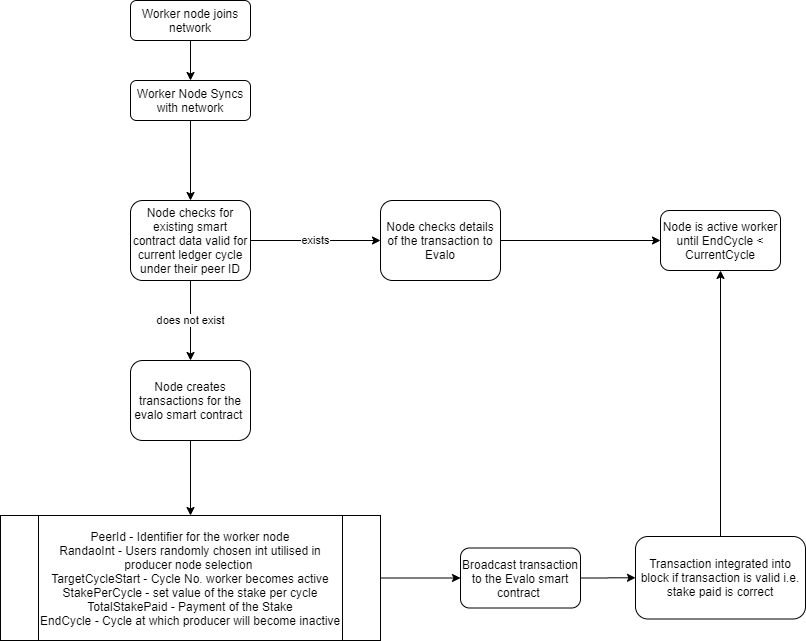
\includegraphics[scale=.40]{Figures/WorkerRegistration.png}

Producer nodes have the ability to determine the length of their service as a producer node as well as which cycles they wish to be eligible to be producer nodes. This thereby gives peers flexibility to how much they invest in their stake, i.e. some workers with access to large amounts of KAT tokens may wish to stake for long periods of time over many cycles, while those with less tokens can become producers for a shorter period of time in order to generate revenue. \\

The smart contract has two specific functions, firstly to keep track of which nodes on the network are valid for selection to become a producer for the proceeding cycle, provide a randomly generated number to determine which of these nodes are in fact selected. These two specific functions have to be deterministic i.e. when the result of the smart contract is calculated on different nodes the same result is calculated. The first part is deterministic to all nodes that in sync with the current state as all transactions to register to become a worker are integrated into a block in the history of the blockchain. The second function is deterministic as for each worker that is eligible to become a producer for a given cycle has supplied a random number from which the global random which determines the producer list for a cycle is derived from. \\

Global random number generation from the smart contract is calculated as follows. Each worker node for cycle $N$ must have registered a transaction to the smart contract at the very latest in cycle $N-1$, contained withing these transactions to the smart contract are random numbers in the range $0~to~2^{256} - 1$. The smart contract calculates the random number through the addition on the modulo point $2^{256} - 1$. For each transactions random number, it is combined with a salt. This salt will be the hash of the previous ledger state update in this cast $\delta = SHA-3(N-1)$. From which for each random number the random output $r = SHA-3(\delta + RandaoInt)$. Each $r$ value for the workers for a given cycle are added together around the modulo point to give a truly random value to give a global random value $G$. This mechanism means that as long as at least one individual is operating fairly the random output can not be manipulated. \\

Each peer ID can only be registered once per cycle. While a producer can have several different entries into the smart contract e.g. cycle $N~to~N+10$ and cycle $N+11~to~N+20$ however these entries can not overlap. Attempt to do so will mean loss of any stake for the crossover and the peer will not be eligible to become a producer for the duplicated cycles. \\

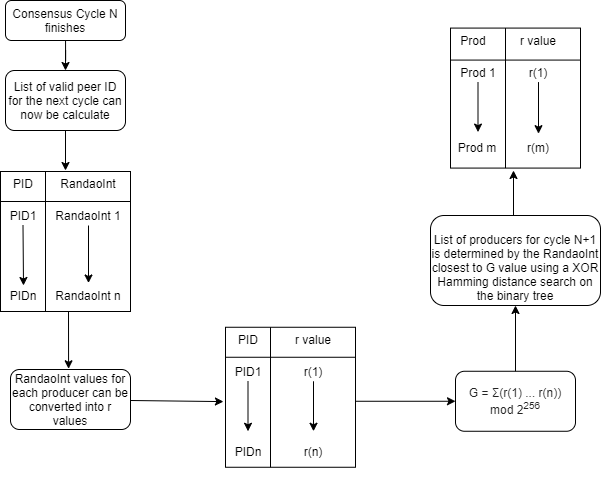
\includegraphics[scale=.45]{Figures/globalRand.png} \\


Every node that is eligible to become a producer for cycle will now have a random value associated with them and there will be a global random number that is created by the smart contract $G$. This is done by determining the nodes that have a $RandaoInt$ closest to the $G$ value using a XOR Hamming distance search on the binary tree. This mechanism gains its security from the fact that all perspective worker nodes are required to declare their random number in advance, and as the random node requires the salt which is determined by the cycle preceding the random values can not be changed or manipulated in any way to give a particular worker any advantage withing the random node selection. \\

This process will allow a verifiable list of N producers, where N is determined by the current amount of registered workers on the network according to security parameters.  

\subsection{Deterministic Threshold Signatures} 

Deterministic threshold signature can be used within the Catalyst consensus algorithm to confirm that only those nodes that have in fact been selected can perform consensus for that give cycle. By secret sharing between the producers that have verifiable been selected to become producers. By secret sharing between the verified nodes in such a way that the public private key pairs of the are required to unlock a given secret, a producer can demonstrate that they are in fact authorised to construct a ledger state update for a given cycle. Through this mechanism, a producer node would be required to sign any ledger state update they release with their element of the key. Any ledger state update would then require a minimum amount of secrets to be added to the ledger state update in order for that ledger state to become `unlocked` and thereby accessible and distributed to all other nodes on the network. 